% =============================================================================
%  TD법 — 『밑바닥부터 시작하는 딥러닝 4』 6장 정리
%
%  컴파일:  xelatex ch06_td.tex  (세 번)
%  (XeLaTeX 계열 엔진 + kotex + NanumGothic 필요)
%  그림:    python ch06/paper/fig_td.py  로 그림 두 개 생성
% =============================================================================
\documentclass[11pt,a4paper]{article}

\usepackage{kotex}
\usepackage{amsmath,amssymb}
\usepackage{amsthm}
\usepackage{graphicx}
\usepackage{booktabs}
\usepackage{multirow}
\usepackage{listings}
\usepackage{xcolor}
\usepackage{algorithm}
\usepackage{algpseudocode}
\usepackage[margin=27mm,top=28mm,bottom=28mm]{geometry}
\usepackage[labelsep=period,font=small,labelfont=bf]{caption}
\usepackage{enumitem}
\usepackage[hidelinks]{hyperref}

% ---- 한글 글꼴 -------------------------------------------------------------
\setmainhangulfont{NanumGothic}
\setsanshangulfont{NanumGothic}
\setmonohangulfont[Scale=MatchLowercase]{NanumGothic}

% ---- 한글 캡션 이름 ---------------------------------------------------------
\renewcommand{\figurename}{그림}
\renewcommand{\tablename}{표}
\renewcommand{\refname}{참고문헌}
\renewcommand{\abstractname}{초록}
\renewcommand{\contentsname}{차례}
\floatname{algorithm}{알고리즘}
\renewcommand{\algorithmicrequire}{\textbf{입력:}}
\renewcommand{\algorithmicensure}{\textbf{출력:}}

% ---- 정리 환경 -------------------------------------------------------------

% ---- 코드 리스팅 -----------------------------------------------------------
\definecolor{codekw}{RGB}{0,86,153}
\definecolor{codecm}{RGB}{112,128,144}
\definecolor{codestr}{RGB}{163,21,21}
\definecolor{codebg}{RGB}{249,249,250}
% 주의: listings는 라틴 문자를 단어 단위로 버퍼링했다가 출력하는데, kotex 환경에서
% 한글이 섞이면 버퍼가 한글 뒤에 flush되어 글자 순서가 뒤바뀐다("q에" -> "에q").
% 그래서 한글 주석은 escapeinside 구간에서 일반 조판 모드로 넘겨 처리한다.
\lstdefinestyle{py}{
  language=Python,
  escapeinside={<@}{@>},
  basicstyle=\ttfamily\small,
  keywordstyle=\color{codekw}\bfseries,
  commentstyle=\color{codecm}\itshape,
  stringstyle=\color{codestr},
  backgroundcolor=\color{codebg},
  frame=single,
  rulecolor=\color{black!25},
  framesep=5pt,
  columns=fullflexible,
  keepspaces=true,
  showstringspaces=false,
  breaklines=true,
  captionpos=b,
  numbers=none,
  aboveskip=1.1em,
  belowskip=0.6em,
}
\lstset{style=py}
\renewcommand{\lstlistingname}{코드}

% ---- 플로트 배치 -----------------------------------------------------------
% 기본값(topfraction 0.7, floatpagefraction 0.5)으로는 표·그림이 본문과 같은 쪽에
% 못 앉고 한데 몰려 '플로트 전용 쪽'을 만든다. 한 쪽이 플로트로 채워질 수 있는 몫을
% 늘리고, 플로트 전용 쪽의 최소 충전율을 올려 성긴 플로트 쪽이 생기지 않게 한다.
\renewcommand{\topfraction}{0.88}
\renewcommand{\bottomfraction}{0.70}
\renewcommand{\textfraction}{0.12}
\renewcommand{\floatpagefraction}{0.80}
\setcounter{topnumber}{3}
\setcounter{bottomnumber}{2}
\setcounter{totalnumber}{5}

% ---- 그림 경로 -------------------------------------------------------------
\graphicspath{{../../images/figures/}{../../images/equations/}{./}}

% ---- 편의 매크로 -----------------------------------------------------------
\newcommand{\E}{\mathbb{E}}
\newcommand{\Sset}{\mathcal{S}}
\newcommand{\Aset}{\mathcal{A}}
\newcommand{\bookfig}[1]{\textit{출처: 원서 그림 #1.}}
\newcommand{\cmt}[1]{\textcolor{codecm}{#1}}   % 리스팅 안의 한글 주석
\newcommand{\Q}{Q}
\DeclareMathOperator*{\argmax}{arg\,max}

% ---- 차례의 절 번호 폭 -------------------------------------------------------
% \thesection 이 "6.1" 처럼 두 토막이라 article 기본 폭(1.5em)으로는 번호와 제목이
% 붙어 버린다. 번호 상자를 넓혀 준다.
\makeatletter
\renewcommand*\l@section[2]{%
  \ifnum \c@tocdepth >\z@
    \addpenalty\@secpenalty
    \addvspace{1.0em \@plus\p@}%
    \setlength\@tempdima{2.8em}%
    \begingroup
      \parindent \z@ \rightskip \@pnumwidth
      \parfillskip -\@pnumwidth
      \leavevmode \bfseries
      \advance\leftskip\@tempdima \hskip -\leftskip
      #1\nobreak\hfil \nobreak\hb@xt@\@pnumwidth{\hss #2}\par
    \endgroup
  \fi}
\renewcommand*\l@subsection{\@dottedtocline{2}{2.8em}{3.4em}}
\makeatother

% ---- 절 번호를 원서 6장 목차에 맞춤 -----------------------------------------
% 번호 있는 절은 원서/README의 6.1~6.6과 정확히 대응한다. 서론과 재현 정보는
% 번호를 붙이지 않고, 하위 절보다 깊은 제목은 번호와 차례에서 뺀다.
\renewcommand{\thesection}{6.\arabic{section}}
\setcounter{secnumdepth}{2}
\setcounter{tocdepth}{2}


\title{\bfseries TD법\\[2mm]
\large 한 걸음의 경험으로 갱신하기: 부트스트래핑, 그리고
정책이 갱신식에서 사라지는 자리}
\author{sajacaros\\\small \texttt{sajacall82@naver.com}}
\date{2026년 9월 10일}

\begin{document}
\maketitle

\begin{abstract}
\noindent
앞 장의 몬테카를로법(MC법)은 환경 모델을 버리고 표본 평균으로 가치를 얻었지만, 수익 $G_t$ 안에
에피소드 끝까지의 보상이 들어 있어 판이 끝나야 한 번 배울 수 있었다. \emph{TD법}(Temporal
Difference)은 기다리지 않는다. 아직 받지 못한 보상의 합을 지금 갖고 있는 추정치 $V(S_{t+1})$로
대신 놓고 한 걸음마다 갱신한다.
본고는 이 한 줄의 교체에서 출발하여 \emph{TD 정책 평가}, \emph{온-정책 제어인 SARSA},
\emph{중요도 샘플링으로 보정하는 오프-정책 SARSA}, \emph{Q 러닝}을 정리하고, 네 알고리즘이
``다음 상태의 값을 누구에게서 받아 오는가''라는 하나의 축 위의 서로 다른 지점임을 보인다.
원서\cite{dlfs4} 6장은 예제 코드를 제공하므로 본고는 그것을 그대로 쓰되, 원서가 관찰로만 남기거나
아예 짚지 않은 다섯 자리에 논의를 더하였다. 절 구성은 원서 6장의 목차를 그대로 따르며, 더한 논의는
그것이 필요해지는 자리의 본문에 ``[보충]''으로 결론만 적고 표와 유도는 부록에 모았다.

\vspace{2mm}
\noindent\textbf{주제어:} 강화 학습, TD법, 부트스트래핑, TD 오차, SARSA, 오프-정책, 중요도 샘플링,
Q 러닝, 벨만 최적 방정식, 분포 모델, 샘플 모델
\end{abstract}

\tableofcontents
\vspace{4mm}

% =============================================================================
\section*{서론}
\addcontentsline{toc}{section}{서론}
% =============================================================================

\subsection*{끝날 때까지 기다리지 않기}

앞 장\cite{ch05}에서 모델을 버리고 표본 평균으로 가치를 얻었다. 갱신식은
\begin{equation*}
  V(S_t) \;\leftarrow\; V(S_t) + \alpha\bigl\{\, G_t - V(S_t) \,\bigr\}
\end{equation*}
이고, 여기에는 $p$도 $r$도 없다. 대신 다른 것이 들어 있다. $G_t$는 $t$부터 에피소드가 끝날 때까지
받은 보상을 전부 더한 값이므로, 이 한 줄을 실행하려면 판이 끝나야 한다. 값이 두 가지다. 판이 길면
갱신이 그만큼 드물어지고, 끝이 없는 \emph{지속적 과제}에는 $G_t$가 정의되지 않아 아예 쓸 수 없다.

이 장은 $G_t$를 기다리지 않는다. 앞 장에서 이미 쓴 재귀 구조 $G_t = R_t + \gamma G_{t+1}$을 다시
꺼내면 모르는 것은 $G_{t+1}$ 하나뿐이고, 그 자리에 지금 갖고 있는 추정치 $V(S_{t+1})$을 넣는다.
\begin{equation*}
  V(S_t) \;\leftarrow\; V(S_t) + \alpha\bigl\{\, R_t + \gamma V(S_{t+1}) - V(S_t) \,\bigr\}.
\end{equation*}
$R_t$와 $S_{t+1}$은 한 걸음만 걸으면 알 수 있으므로 갱신이 걸음마다 일어난다. 아직 부정확한
추정치를 목표로 삼아 다른 추정치를 고치는 이 방식을 \emph{부트스트래핑}이라 하며, 앞 장의 DP도 같은
성격이었다. 교체의 대가는 편향이다. $G_t$는 참값 주위에 고르게 흩어지지만
$R_t + \gamma V(S_{t+1})$은 $V$가 틀린 만큼 한쪽으로 치우친 값이다. 대신 얻는 것이 작은 분산과
잦은 갱신이다.

제어로 넘어가면 두 번째 소득이 나온다. 앞 장에서 오프-정책의 약점이던 중요도 가중치의 긴 곱은 한
걸음만 내다보는 TD법에서 곱 하나로 끝나고, 다음 상태의 값을 ``실제로 고른 행동의 $Q$'' 대신
``$\max_a Q$''로 바꾸면 정책이 갱신식에서 통째로 사라져 보정할 것 자체가 없어진다. 3장에서 벨만
방정식과 벨만 최적 방정식을 가르던 $\sum_a \pi(a\mid s)$ 대 $\max_a$의 차이가 여기서 알고리즘의
차이로 나타난다.

\subsection*{본고의 구성과 기여}

본고는 원서 6장의 목차를 그대로 따른다. 벨만 방정식을 기댓값 모양 그대로 두고 표본 하나로 바꾸어
TD법을 도출해 정책 평가에 쓰고, 평가 대상을 $V$에서 $Q$로 옮겨 온-정책 제어인 SARSA를 만든다. 이어
걷는 정책과 평가받는 정책을 갈라 한 걸음분 중요도 가중치로 보정하고, 다음 상태의 값을 $\max_a Q$로
바꾸어 그 가중치마저 없애는 Q 러닝에 이른다. 마지막으로 정책을 확률분포로 들고 있을 필요가 없다는
것을 확인해 코드를 $Q$ 하나로 줄인다.

원서 6장은 예제 코드를 제공하므로 본고는 그것을 그대로 쓰되, 원서가 관찰로만 남기거나 아예 짚지 않은
다섯 자리에 논의를 더하였다. 더한 논의는 그것이 필요해지는 자리의 본문에 ``[보충]''으로 표시하고
결론만 몇 줄로 적었으며, 그것을 떠받치는 표와 유도는 부록에 모았다. 줄거리를 따라가는 독자는 [보충]만
읽고 지나가면 되고, 근거가 궁금한 자리에서만 부록을 펼치면 된다.

수렴 정리의 증명, TD($\lambda$)와 적격 흔적, 최대화 편향과 이중 Q 러닝 같은 대목은 이 장의 줄거리를
따라가는 데 꼭 필요하지 않아 덜어냈다.

% =============================================================================
\section{TD법으로 정책 평가하기}
\label{sec:eval}
% =============================================================================

\subsection{TD법 도출}
\label{sec:derive}

앞의 두 장이 가치 함수를 구한 방식은 백업 다이어그램의 어디를 쓰느냐로 갈린다.

\begin{figure}[htbp]
\centering
\includegraphics[width=0.86\linewidth]{{fig 6-1}.png}
\caption{DP법(왼쪽)과 MC법(오른쪽)이 쓰는 범위. 왼쪽은 폭이 넓고 깊이가 한 층이다. 다음 상태를
빠짐없이 훑되 한 걸음만 내려가며, 전부 훑으려면 $p$와 $\pi$를 알아야 한다. 오른쪽은 폭이 한 줄기고
깊이가 끝까지다. 모델은 필요 없지만 바닥에 닿아야, 곧 에피소드가 끝나야 값이 나온다. \bookfig{6-1}}
\label{fig:dp-mc}
\end{figure}

두 방법의 제약이 서로 다른 축에서 온다. DP의 제약은 폭에 있고 MC의 제약은 깊이에 있다. 그러면 폭도
한 줄기, 깊이도 한 층으로 두면 둘 다 피할 수 있다.

\begin{figure}[htbp]
\centering
\includegraphics[width=0.44\linewidth]{{fig 6-2}.png}
\caption{TD법이 쓰는 범위. 한 줄기만 겪으므로 모델이 필요 없고, 한 층에서 멈추므로 에피소드가
끝나기를 기다리지 않는다. 잘라 낸 아래쪽은 지금 갖고 있는 추정치 $V(S_{t+1})$로 대신한다.
\bookfig{6-2}}
\label{fig:td-idea}
\end{figure}

식으로 따라가면 출발점은 3장의 재귀 구조다.
\begin{equation*}
  G_t = R_t + \gamma R_{t+1} + \gamma^2 R_{t+2} + \cdots = R_t + \gamma G_{t+1}.
\end{equation*}
가치 함수의 정의 $v_\pi(s) = \E_\pi[G_t \mid S_t = s]$에 넣으면
\begin{equation*}
  v_\pi(s) = \E_\pi\bigl[\, R_t + \gamma G_{t+1} \mid S_t = s \,\bigr]
           = \E_\pi\bigl[\, R_t + \gamma v_\pi(S_{t+1}) \mid S_t = s \,\bigr]
\end{equation*}
가 된다. 두 번째 등호에서 $G_{t+1}$이 $v_\pi(S_{t+1})$로 바뀐 것은 조건부 기댓값을 한 번 더 취한
것이며, 이 식이 3장의 벨만 방정식이다.

여기서 길이 갈린다. 기댓값을 확률로 펼쳐 쓰면
\begin{equation*}
  v_\pi(s) = \sum_a \pi(a\mid s) \sum_{s'} p(s'\mid s,a)
             \bigl\{\, r(s,a,s') + \gamma\, v_\pi(s') \,\bigr\}
\end{equation*}
이고, 등호를 갱신식으로 바꿔 읽은 것이 앞 장의 반복적 정책 평가였다. 우변에 $\pi$와 $p$가 그대로
남아 있어 모델을 알아야만 계산된다. 펼치지 않고 기댓값 모양 그대로 두면 사정이 다르다. 우변에 $p$도
$\pi$도 없고 기댓값 기호만 남아 있으니, 앞 장에서 배운 대로 표본의 평균으로 근사할 수 있다. 표본
하나는 실제로 한 걸음 걸어서 얻은 $R_t + \gamma V(S_{t+1})$이다.

\begin{figure}[htbp]
\centering
\includegraphics[width=0.80\linewidth]{{fig 6-3}.png}
\caption{두 갱신식에서 다른 곳은 하늘색으로 칠한 자리 하나뿐이다. MC법은 실제로 받은 수익 $G_t$를,
TD법은 한 걸음 뒤에 곧바로 알 수 있는 $R_t + \gamma V(S_{t+1})$을 목표로 삼는다. \bookfig{6-3}}
\label{fig:mc-vs-td-eq}
\end{figure}

\begin{align*}
  \text{MC법:}\quad & V(S_t) \leftarrow V(S_t) + \alpha\bigl\{\, G_t - V(S_t) \,\bigr\},\\
  \text{TD법:}\quad & V(S_t) \leftarrow V(S_t) + \alpha\bigl\{\, \underbrace{R_t + \gamma V(S_{t+1})}_{\text{TD 목표}} - V(S_t) \,\bigr\}.
\end{align*}
$R_t + \gamma V(S_{t+1})$을 \emph{TD 목표}, 중괄호 전체
$R_t + \gamma V(S_{t+1}) - V(S_t)$를 \emph{TD 오차}라 한다.

아직 부정확한 $V(S_{t+1})$을 목표로 삼아 $V(S_t)$를 고치는 것이 이상해 보이지만, 매 걸음
$R_t$라는 실제로 받은 값이 조금씩 섞여 들어온다. 잘못된 추정치끼리 서로를 참조하는 것이 아니라
진짜 정보가 한 걸음씩 뒤로 스며드는 구조이며, 앞 장의 DP도 같은 방식으로 참값에 다가갔다.

\subsection{MC법과 TD법 비교}
\label{sec:compare}

두 목표값의 성질이 갈리는 곳은 흩어진 정도다.

\begin{figure}[htbp]
\centering
\includegraphics[width=0.72\linewidth]{{fig 6-4}.png}
\caption{같은 자리에서 출발한 자동차의 경로가 시간이 갈수록 부채꼴로 벌어진다. 왼쪽 점선까지의
결과는 폭이 좁고 오른쪽 점선까지 가면 크게 흩어진다. $G_t$는 오른쪽 점선까지 간 값이고
$R_t + \gamma V(S_{t+1})$은 왼쪽 점선까지만 간 값이다. \bookfig{6-4}}
\label{fig:variance-fan}
\end{figure}

$G_t$에는 에피소드가 끝날 때까지 고른 행동과 겪은 전이의 무작위성이 전부 쌓인다. 앞 장에서
$3\times4$ 그리드 월드의 한 에피소드가 평균 $44.8$걸음이었으니 $G_t$ 하나에 $45$번의 뽑기가 들어
있는 셈이다. TD 목표에 들어 있는 무작위성은 $R_t$와 $S_{t+1}$, 곧 한 번의 뽑기뿐이다.

\begin{table}[htbp]
\centering
\caption{두 목표값의 성질. 편향과 분산을 실제로 갈라 잰 것은 이 절 끝의 [보충]에 있다.}
\label{tab:mc-td}
\small
\begin{tabular}{@{}lll@{}}
\toprule
 & MC법 & TD법 \\
\midrule
목표값        & $G_t$                        & $R_t + \gamma V(S_{t+1})$ \\
언제 알 수 있나 & 에피소드가 끝난 뒤            & 한 걸음 뒤 \\
편향          & 없음                          & 있음($V$가 부정확한 만큼) \\
분산          & 큼(끝까지의 무작위성이 쌓임)    & 작음(한 걸음분) \\
지속적 과제    & 쓸 수 없음                    & 쓸 수 있음 \\
\bottomrule
\end{tabular}
\end{table}

편향과 분산 가운데 무엇을 줄일지 고르는 저울이며, 갱신이 잦다는 점까지 더해 실무에서는 대체로
TD법이 앞선다.

\subsection{TD법 구현}
\label{sec:td-impl}

\begin{lstlisting}[caption={TD 정책 평가 (\texttt{s01\_td\_eval.py}), $\alpha=0.01$},label={lst:td-eval}]
def eval(self, state, reward, next_state, done):
    next_V = 0 if done else self.V[next_state]   <@\cmt{\# 목표 지점의 가치는 0}@>
    target = reward + self.gamma * next_V        <@\cmt{\# TD 목표}@>
    self.V[state] += (target - self.V[state]) * self.alpha
\end{lstlisting}

\lstinline|done|일 때 \lstinline|next_V|를 $0$으로 두는 것은 종료 상태 다음으로는 받을 보상이 없기
때문이다. 종료 상태의 가치는 정의상 $0$이다.

앞 장과 갈리는 자리는 갱신식이 아니라 호출 위치에 있다.

\begin{lstlisting}[caption={실행 루프. \lstinline|agent.eval()|이 \lstinline|if done| \emph{바깥}에 있다},label={lst:td-loop}]
while True:
    action = agent.get_action(state)
    next_state, reward, done = env.step(action)

    agent.eval(state, reward, next_state, done)   <@\cmt{\# 걸음마다 부른다}@>
    if done:
        break
    state = next_state
\end{lstlisting}

앞 장 \texttt{ch05/s02\_mc\_eval.py}에서는 같은 자리의 호출이 \lstinline|if done:| 안에 있었다.
한 걸음 정보만으로 갱신이 끝나므로 \lstinline|memory|도 사라졌다. 에피소드를 통째로 들고 있을
이유가 없어진 것이 TD법이 코드에 남기는 가장 눈에 띄는 흔적이다.

\begin{figure}[htbp]
\centering
\includegraphics[width=0.52\linewidth]{{fig 6-5}.png}
\caption{$1{,}000$ 에피소드를 돌린 뒤의 가치 함수. 앞 장 그림 5-12(MC법), 그 앞 장 그림 4-13(DP)과
거의 같은 그림이 나온다. 세 방법이 같은 정책을 평가하므로 답이 같아야 하고, 다른 것은 오차뿐이다.
\bookfig{6-5}}
\label{fig:td-result}
\end{figure}

시드 $50$개로 재면 $v_\pi$에 대한 RMSE가 $0.0376$이다. $\alpha$를 $0.01$로 작게 잡은 것은 갱신
횟수가 많기 때문이다. 한 에피소드에 한 번씩 갱신하던 앞 장과 달리 걸음마다 갱신하므로 $1{,}000$
에피소드에서 갱신이 수만 번 일어난다. $\alpha$를 크게 잡으면 앞 장에서 본 잔차 띠가 그만큼 넓어져
값이 출렁인다.

\subsubsection{[보충] 편향과 분산을 갈라 보기}
\label{sec:bias-var}

원서는 편향이 TD법에 있고 분산이 MC법에 있다고 적을 뿐 어느 쪽이 얼마인지는 적지 않는다. 같은
궤적을 세 갱신식에 똑같이 먹이고 시드 $60$개에서 두 양을 따로 재면 표가 그대로 확인된다.
$1{,}000$ 에피소드에서 TD법의 표준편차는 $0.0295$이고 $\alpha$를 맞춘 MC법은 $0.0924$로 세 배가
넘게 벌어진다. TD 목표에는 한 걸음분의 무작위성만 들어 있고 $G_t$에는 평균 $44.8$걸음분이 쌓인다는
사실이 숫자로 나온 것이다.

편향은 초반에만 보인다. $250$ 에피소드에서 TD법의 편향이 $0.0749$로 MC법의 다섯 배 가까이 큰데,
$V$가 아직 초깃값 $0$ 근처에 있어 TD 목표가 통째로 작게 나오기 때문이다. $1{,}000$ 에피소드에서
$0.0044$까지 떨어져 MC법과 같은 수준이 된다. 부트스트래핑의 편향은 $V$가 채워지면서 스스로 걷힌다.
원서가 표로 적은 두 성질은 둘 다 사실이지만 유효 기간이 다른 셈이다. 분산의 차이는 학습이 끝날
때까지 남고, 편향의 차이는 초반 몇백 에피소드에서만 보인다.

한 가지가 더 보인다. TD법의 RMSE가 $1{,}000$ 에피소드부터 $0.036$ 근처에서 더 내려가지 않는다. 앞
장에서 본 고정값 $\alpha$의 잔차 띠이며, MC법도 $\alpha=0.01$을 쓰면 $0.098$에서 똑같이 멈춘다.
반면 $1/n$ 평균은 $8{,}000$ 에피소드까지 계속 내려가 $0.0094$에 이른다. 그래서 예제가 쓰는
설정끼리, 곧 TD법($\alpha=0.01$)과 앞 장의 MC법($1/n$)을 그대로 견주면 $1{,}000$ 에피소드에서
$0.0358$ 대 $0.0229$로 MC법이 앞선다. TD법이 진 것이 아니라 고정값 $\alpha$가 $1/n$ 평균에 진
것이다. 에피소드별 실측은 부록~\ref{app:bias-var}에 있다.

% =============================================================================
\section{SARSA}
\label{sec:sarsa}
% =============================================================================

\subsection{온-정책 SARSA}
\label{sec:sarsa-derive}

평가에 개선을 붙이면 제어가 된다. 앞 장 5.4.1절에서 확인했듯 모델이 없으면 탐욕화에 쓸 수 있는
것은 $\argmax_a Q(s,a)$뿐이므로, 평가의 대상도 $V$가 아니라 $Q$여야 한다. TD 갱신식의 $V$를 $Q$로
바꾸면 그대로 옮겨진다.
\begin{equation*}
  Q(S_t,A_t) \;\leftarrow\; Q(S_t,A_t)
    + \alpha\bigl\{\, R_t + \gamma Q(S_{t+1},A_{t+1}) - Q(S_t,A_t) \,\bigr\}.
\end{equation*}

\begin{figure}[htbp]
\centering
\includegraphics[width=0.56\linewidth]{{fig 6-6}.png}
\caption{갱신에 필요한 것을 시간 순으로 늘어놓은 것. $S_t$, $A_t$, $R_t$, $S_{t+1}$, $A_{t+1}$
다섯이며, 머리글자를 따서 \emph{SARSA}라 부른다. 오른쪽 끝의 $A_{t+1}$까지 정해져야 갱신할 수
있으므로 갱신이 한 걸음 늦게 일어난다. \bookfig{6-6}}
\label{fig:sarsa-name}
\end{figure}

개선 쪽은 앞 장과 같은 $\varepsilon$-탐욕 정책이다.
\begin{equation*}
  \pi(a \mid s) =
  \begin{cases}
    \dfrac{\varepsilon}{|\Aset|} + 1 - \varepsilon & a = \argmax_{a'} Q(s,a'),\\[6pt]
    \dfrac{\varepsilon}{|\Aset|} & \text{그 밖의 행동}.
  \end{cases}
\end{equation*}
SARSA는 위의 평가와 개선을 걸음마다 번갈아 한다. 앞 장의 MC 제어가 에피소드마다 번갈아 하던 것을
한 걸음 단위로 잘게 쪼갠 것이며, 앞 장에서 \emph{일반화된 정책 반복}이라 부른 틀 안에서 더 극단으로
간 지점이다.

\subsection{SARSA 구현}
\label{sec:sarsa-impl}

\begin{lstlisting}[caption={SARSA (\texttt{s02\_sarsa.py}), $\alpha=0.8$, $\varepsilon=0.1$},label={lst:sarsa}]
self.memory = deque(maxlen=2)          <@\cmt{\# 최근 두 걸음만 보관}@>

def update(self, state, action, reward, done):
    self.memory.append((state, action, reward, done))
    if len(self.memory) < 2:           <@\cmt{\# 아직 A\_\{t+1\}을 모른다}@>
        return

    state, action, reward, done = self.memory[0]
    next_state, next_action, _, _ = self.memory[1]
    next_q = 0 if done else self.Q[next_state, next_action]

    target = reward + self.gamma * next_q                       <@\cmt{\# 평가}@>
    self.Q[state, action] += (target - self.Q[state, action]) * self.alpha
    self.pi[state] = greedy_probs(self.Q, state, self.epsilon)  <@\cmt{\# 개선}@>
\end{lstlisting}

앞 장의 \lstinline|memory|가 에피소드 전체를 담았던 것과 달리 여기서는 길이 $2$면 충분하다.
\lstinline|deque(maxlen=2)|는 새 데이터를 넣으면 가장 오래된 것을 자동으로 밀어낸다. 목표에
도달했을 때 \lstinline|agent.update(next_state, None, None, None)|을 한 번 더 부르는 것도 그
구조에서 나온다. 마지막 걸음은 \lstinline|memory|에 하나만 들어 있어 갱신되지 못하므로, 더미를
밀어 넣어 마지막 $(S,A)$까지 갱신되게 한다.

\begin{figure}[htbp]
\centering
\includegraphics[width=\linewidth]{{fig 6-7}.png}
\caption{$10{,}000$ 에피소드로 학습한 $Q$ 함수(왼쪽)와 그것을 탐욕화한 정책(오른쪽). 원서는
아래 줄의 왼쪽 화살표 셋에 ``폭탄에서 멀어지는 행동''이라 적어 두었다. 셋 가운데 오른쪽 끝
$(2,3)$의 \texttt{LEFT}는 최적 정책과 같지만 $(2,1)$과 $(2,2)$는 다르며, 그 두 칸이 왜 그렇게
되는지는 이 절 끝의 [보충]에서 다룬다. \bookfig{6-7}}
\label{fig:sarsa-result}
\end{figure}

성적은 앞 장의 MC 제어보다 나쁘다. 시드 $50$개에서 최적 행동 일치가 $7.62/10$이고 $10$칸을 모두
맞힌 시드가 하나도 없다. 한 걸음마다 갱신하니 더 나아야 할 것 같은데 그렇지 않다. 원인의 일부는
평가 대상에 있다. 앞 장에서 본 대로 온-정책 제어가 다가가는 값은 $v_*$가 아니라
$\varepsilon$-탐욕 정책 자신의 가치이므로 $v_*$보다 아래다. 그러나 그 몫은 $\varepsilon=0.1$에서
평균 $-0.0235$였고, 여기서 관찰된 치우침 $-0.1409$의 $6$분의 $1$에 지나지 않는다. 나머지는
$\alpha$에서 온다.

\subsubsection{[보충] 그림 \ref{fig:sarsa-result}의 화살표는 안전한 길이 아니다}
\label{sec:sarsa-alpha}

원서는 그림~\ref{fig:sarsa-result} 아래 줄의 왼쪽 화살표를 이렇게 읽는다. SARSA가 평가하는 것은
$\varepsilon$만큼 헤매는 자기 자신이므로, 폭탄 옆을 지나는 길을 고르면 열 번에 한 번은 실수로
폭탄에 빠지고 그 손해가 $Q$에 반영되어 안전하지만 돌아가는 길을 고른다는 설명이다.

설명이 맞다면 $\varepsilon$-탐욕 정책의 가치를 정확히 계산했을 때도 그 자리의 최선이 \texttt{LEFT}
여야 한다. SARSA가 수렴하는 대상은 $\varepsilon$-소프트 정책 가운데 가치가 가장 높은 것이므로, 앞
장의 정책 반복법을 $\varepsilon$-소프트 정책으로 제한해 돌리면 그 값을 표본 없이 얻을 수 있다.
그렇게 계산하면 예제가 쓰는 $\varepsilon=0.1$에서 문제의 칸 $(2,2)$의 최선은 \texttt{UP}이고
\texttt{LEFT}보다 $0.16$ 앞선다. $\varepsilon$을 $0.5$까지 올려도 순서가 바뀌지 않으며, 위험
회피가 실제로 정책을 뒤집으려면 $\varepsilon$이 $0.9$는 되어야 한다.

이 환경에서 위험이 작은 까닭은 폭탄의 처지에 있다. 폭탄 칸 $(1,3)$은 밟아도 에피소드가 끝나지 않고
목표 바로 아래에 있다. 실수로 들어가면 $-1$을 받지만 곧바로 위로 올라가 $+1$을 받으므로 손해가
$-1 + \gamma \cdot 1.0 = -0.1$에 그친다. 낭떠러지에서 떨어지면 출발점으로 돌아가는 교과서의 예제와
성질이 다르다.

그러면 화살표는 어디서 오는가. 경험을 $20$배로 늘려도 $(2,2)$에서 \texttt{UP}을 고른 시드가
$2/20$ 그대로다. 표본이 모자란 것이 아니다. $\alpha$를 $0.1$로 낮추면 같은 $10{,}000$ 에피소드에서
$17/20$로 뒤집힌다. 범인은 $\alpha=0.8$이다. 앞 장에서 고정값 $\alpha$가 추정치를 한 점에 모으지
못하고 폭 $\sqrt{\alpha/(2-\alpha)}\,\sigma$의 띠 안에 남긴다는 것을 보았는데, $\alpha=0.8$이면
계수가 $0.8165$로 앞 장이 쓰던 $\alpha=0.1$의 $0.2294$보다 세 배 넘게 크다. 실제로 $(2,2)$에서
값이 머무는 자리의 표준편차를 재면 $0.2381$이고, 두 행동의 차이 $0.16$이 그 안에 묻힌다.

그리고 그 흔들림은 스스로를 키운다. 값이 낮게 찍힌 칸은 정책이 등을 돌리고, 등을 돌리면 덜
방문되며, 덜 방문되면 값이 그대로 남는다. 방문 횟수가 시작 칸 $14{,}271$번 대 $(2,2)$ $378$번으로
$38$배 벌어지는 것이 그 고리의 결과이며, $\alpha$를 낮추면 $(2,2)$ 방문이 $6{,}089$번으로 $16$배
늘어난다. $\varepsilon$-소프트 최적 가치, 원인을 갈라 본 표, 잔차 띠의 계산은
부록~\ref{app:sarsa-alpha}에 있다.

원서가 $\alpha=0.8$을 고른 데는 이유가 있다. 뒤에 나올 Q 러닝에서는 이 값이 문제를 일으키지 않으며
오히려 빠른 학습에 도움이 되는데, 같은 $\alpha$가 두 알고리즘에서 갈리는 까닭은 Q 러닝의 TD 목표에
분산이 없다는 데 있다.

% =============================================================================
\section{오프-정책 SARSA}
\label{sec:offsarsa}
% =============================================================================

\subsection{오프-정책과 중요도 샘플링}
\label{sec:off-motive}

동기는 앞 장 5.5절과 같다. 탐색은 $\varepsilon$-탐욕 정책 $b$에 맡기고 평가는 탐욕 정책 $\pi$에
대해 하고 싶다. 그렇게 하면 앞 절에서 본 $\varepsilon$ 몫이 사라진다. 먼저 갱신식에서 확률이
개입하는 자리를 찾는다.

\begin{figure}[htbp]
\centering
\includegraphics[width=0.62\linewidth]{{fig 6-8}.png}
\caption{SARSA 갱신식에서 뽑기가 일어나는 두 자리. $S_t \to R_t, S_{t+1}$은 환경의
$p(s'\mid s,a)$이고 바꿀 수 없다. $S_{t+1} \to A_{t+1}$은 정책이며, 데이터를 모은 것은 $b$인데
평가하고 싶은 것은 $\pi$라 어긋나는 자리가 여기다. \bookfig{6-8}}
\label{fig:sarsa-backup-prob}
\end{figure}

환경 쪽 뽑기는 어느 정책을 쓰든 같으므로 보정할 것이 없다. 남는 것은 $A_{t+1}$ 하나다.
$A_{t+1} \sim \pi$로 뽑혔다면 지금까지의 온-정책 SARSA이고, $b$로 뽑혔다면 앞 장의 중요도
가중치로 보정한다.
\begin{equation*}
  \rho = \frac{\pi(A_{t+1} \mid S_{t+1})}{b(A_{t+1} \mid S_{t+1})},
  \qquad A_{t+1} \sim b.
\end{equation*}

$\rho$가 \emph{한 걸음분}이라는 것이 앞 장과 갈리는 결정적인 자리다. 앞 장의 MC법에서는 종료까지의
가중치를 전부 곱해 쌓아야 했고, 곱이 길어질수록 $0$으로 꺼지거나 폭발하는 것이 고질적인 약점이었다.
TD법은 한 걸음만 내다보므로 곱이 하나로 끝난다. 곱이 길어지지 않는 덕에 TD법은 오프-정책과 잘 맞는다.

\subsection{오프-정책 SARSA 구현}
\label{sec:off-impl}

\begin{lstlisting}[caption={오프-정책 SARSA (\texttt{s03\_sarsa\_off\_policy.py}), $\alpha=0.8$, $\varepsilon=0.1$},label={lst:off-sarsa}]
if done:
    next_q = 0
    rho = 1
else:
    next_q = self.Q[next_state, next_action]
    rho = self.pi[next_state][next_action] / self.b[next_state][next_action]

target = rho * (reward + self.gamma * next_q)      <@\cmt{\# rho로 TD 목표 보정}@>
self.Q[state, action] += (target - self.Q[state, action]) * self.alpha

self.pi[state] = greedy_probs(self.Q, state, 0)            <@\cmt{\# 대상 정책: 탐욕}@>
self.b[state] = greedy_probs(self.Q, state, self.epsilon)  <@\cmt{\# 행동 정책: eps-탐욕}@>
\end{lstlisting}

\lstinline|rho|가 \lstinline|*=|가 아니라 매번 새로 계산된다는 점이 앞 장과 다르다. 앞 장의
\lstinline|update()|에는 \lstinline|rho *= ...|가 있었고 그 한 글자가 분산의 근원이었다.

\begin{figure}[htbp]
\centering
\includegraphics[width=\linewidth]{{fig 6-9}.png}
\caption{오프-정책 SARSA의 결과. 그림~\ref{fig:sarsa-result}와 견주면 폭탄 칸 $(1,3)$이
\texttt{UP}으로 목표를 향하고 $Q$ 값도 전반적으로 크다. 평가 대상이 헤매지 않는 탐욕 정책이라
실수로 폭탄에 빠지는 몫을 셈하지 않기 때문이다. \bookfig{6-9}}
\label{fig:off-sarsa-result}
\end{figure}

앞 장 5.5절에서 본 것과 같은 모양이 나온다. 정책은 더 잘 맞히고(최적 행동 $7.62 \to 8.36$칸,
$10$칸을 모두 맞힌 시드 $0\% \to 22\%$) 값은 더 못 맞힌다(RMSE $0.2475 \to 0.2885$). 평가 대상이
탐욕 정책으로 바뀌어 $\varepsilon$ 몫이 사라지는 대신 $\rho$가 목표를 흔든다.

\subsubsection{[보충] \texorpdfstring{$\rho$}{rho}를 곱하는 자리}
\label{sec:rho-place}

예제의 목표는 $\rho\,(R_t + \gamma Q')$로, 괄호 안에 보상 $R_t$가 함께 들어가 있다. 교과서가 쓰는
형태는 다르다.
\begin{equation*}
  \text{예제:}\quad \rho\bigl(R_t + \gamma Q(S_{t+1},A_{t+1})\bigr),
  \qquad
  \text{교과서\cite{sutton}:}\quad R_t + \gamma\,\rho\,Q(S_{t+1},A_{t+1}).
\end{equation*}
$\rho$가 보정하려는 것은 $A_{t+1}$을 어느 정책으로 뽑았느냐이고, $R_t$는 $A_{t+1}$이 정해지기
전에 이미 받은 값이라 보정 대상이 아니다. 그래서 교과서 형태에서는 $\rho$가 다음 상태의 값에만
붙는다. 예제 형태에서는 $\rho=0$일 때 목표가 통째로 $0$이 되어 실제로 받은 보상까지 지워진다.

그런데 같은 조건에서 견주면 두 형태의 차이가 시드 사이의 흔들림에 묻힌다. 까닭은 두 가지다. 먼저
한 걸음짜리 $\rho$가 $0$이 되는 것은 갱신의 $6.99\%$뿐이다. 앞 장 MC법에서 같은 값이 $59.9\%$
였던 것과 크게 다른데, 앞 장에서는 누적곱이라 한 걸음만 어긋나도 그보다 앞선 걸음이 전부 죽었기
때문이다. 그리고 두 형태가 실제로 갈리는 것은 $\rho=0$이면서 보상이 $0$이 아닌 갱신뿐인데, 그런
갱신이 $136{,}813$회 가운데 $23$회다. 이 환경은 보상이 목표 칸과 폭탄 칸에서만 나오고 나머지
$10$칸에서는 모두 $0$이라 두 형태가 만날 기회 자체가 드물다. 보상이 걸음마다 나오는 환경이라면
차이가 드러날 것이며, 그때는 교과서 형태를 써야 한다. 두 형태의 성적과 $\rho$가 실제로 취한 값의
분포는 부록~\ref{app:rho-place}에 있다.

% =============================================================================
\section{Q 러닝}
\label{sec:qlearning}
% =============================================================================

오프-정책 SARSA는 여전히 $\rho$를 들고 다닌다. 그것마저 없앨 수 있는지가 이 절의 질문이며, 답은
3장의 두 방정식에 있다.

\begin{figure}[htbp]
\centering
\includegraphics[width=0.56\linewidth]{{fig 6-10}.png}
\caption{이 절의 결론. 벨만 방정식을 표본으로 바꾸면 SARSA가 되고, 벨만 최적 방정식을 표본으로
바꾸면 Q 러닝이 된다. 3장에서 두 방정식을 가르던 것은 $\sum_a \pi(a\mid s)$와 $\max_a$의 차이
하나였다. \bookfig{6-10}}
\label{fig:two-equations}
\end{figure}

\subsection{벨만 방정식과 SARSA}
\label{sec:bellman-sarsa}

\begin{figure}[htbp]
\centering
\begin{minipage}[t]{0.48\linewidth}\centering
  \includegraphics[width=\linewidth]{{fig 6-11}.png}
\end{minipage}\hfill
\begin{minipage}[t]{0.48\linewidth}\centering
  \includegraphics[width=\linewidth]{{fig 6-12}.png}
\end{minipage}
\caption{왼쪽: $Q$ 함수에 대한 벨만 방정식의 백업 다이어그램. 갈래가 두 번 퍼지며, 한 번은
$p(s'\mid s,a)$로 다른 한 번은 $\pi(a\mid s)$로 퍼진다. 정확히 계산하려면 두 갈래를 모두 훑어야
하므로 모델이 필요하다. 오른쪽: 두 갈래에서 각각 한 줄기씩 뽑은 것이 SARSA다. \bookfig{6-11, 6-12}}
\label{fig:bellman-backup}
\end{figure}

벨만 방정식이 퍼뜨리는 두 갈래에서 각각 한 줄기씩 뽑은 것이 SARSA이며, 그래서 SARSA를 벨만
방정식의 표본 판본이라 부른다. 문제도 거기서 나온다. $\pi(a\mid s)$에서 뽑아야 하는데 실제로 걷는
것은 $b$다. 오프-정책으로 만들려면 $\rho$로 그 어긋남을 메워야 했다.

\subsection{벨만 최적 방정식과 Q 러닝}
\label{sec:bellman-opt}

\begin{figure}[htbp]
\centering
\begin{minipage}[t]{0.50\linewidth}\centering
  \includegraphics[width=\linewidth]{{fig 6-13}.png}
\end{minipage}\hfill
\begin{minipage}[t]{0.46\linewidth}\centering
  \includegraphics[width=\linewidth]{{fig 6-14}.png}
\end{minipage}
\caption{왼쪽: 벨만 최적 방정식의 백업 다이어그램. 마지막 층이 확률적 선택이 아니라 \texttt{MAX}
이고 회색으로 흐려진 가지는 버려진다. 오른쪽: 그것을 표본으로 바꾼 것. 뽑기 표시가 한 군데뿐이며,
$\max_a Q(S_{t+1},a)$는 이미 갖고 있는 $Q$ 표를 훑어 얻으므로 뽑기가 아니다. \bookfig{6-13, 6-14}}
\label{fig:bellman-opt-backup}
\end{figure}

마지막 층에서 정책이 사라졌다는 것이 전부다. 식에 $\pi$도 $b$도 등장하지 않으니 어긋날 것이 없고,
어긋나지 않으니 보정할 것도 없다. $\rho$가 필요 없어진다.
\begin{equation*}
  Q(S_t,A_t) \;\leftarrow\; Q(S_t,A_t)
    + \alpha\bigl\{\, R_t + \gamma \max_{a} Q(S_{t+1},a) - Q(S_t,A_t) \,\bigr\}.
\end{equation*}
SARSA의 갱신식과 다른 곳은 $Q(S_{t+1},A_{t+1})$이 $\max_a Q(S_{t+1},a)$로 바뀐 자리 하나다.

\begin{table}[htbp]
\centering
\caption{다음 상태의 값을 어디서 받아 오는가. 세 알고리즘의 차이가 그 한 열에서 갈린다.}
\label{tab:three-updates}
\small
\begin{tabular}{@{}llll@{}}
\toprule
 & 다음 상태의 값 & 갱신에 필요한 것 & 성격 \\
\midrule
SARSA           & 실제로 고른 $A_{t+1}$의 $Q$ & $A_{t+1}$              & 온-정책 \\
오프-정책 SARSA & 같음 + $\rho$ 보정          & $A_{t+1}$, $\pi$, $b$  & 오프-정책 \\
Q 러닝          & $\max_a Q(S_{t+1},a)$       & 없음                   & 오프-정책, 보정 불필요 \\
\bottomrule
\end{tabular}
\end{table}

$A_{t+1}$을 기다릴 필요가 없어져 갱신이 한 걸음 안에서 끝나고, 코드에서 \lstinline|deque|가
사라진다.

\subsection{Q 러닝 구현}
\label{sec:q-impl}

\begin{lstlisting}[caption={Q 러닝 (\texttt{s04\_q\_learning.py}), $\alpha=0.8$, $\varepsilon=0.1$},label={lst:qlearning}]
def update(self, state, action, reward, next_state, done):
    if done:
        next_q_max = 0
    else:
        next_qs = [self.Q[next_state, a] for a in range(self.action_size)]
        next_q_max = max(next_qs)          <@\cmt{\# SARSA와 다른 단 한 곳}@>

    target = reward + self.gamma * next_q_max
    self.Q[state, action] += (target - self.Q[state, action]) * self.alpha

    self.pi[state] = greedy_probs(self.Q, state, epsilon=0)     <@\cmt{\# 대상 정책}@>
    self.b[state] = greedy_probs(self.Q, state, self.epsilon)   <@\cmt{\# 행동 정책}@>
\end{lstlisting}

\begin{figure}[htbp]
\centering
\includegraphics[width=\linewidth]{{fig 6-15}.png}
\caption{Q 러닝의 결과. $Q$ 값이 $1.00$, $0.90$, $0.81$, $0.73$, $0.66$처럼 $\gamma$의 거듭제곱으로
정확히 찍히고, 폭탄으로 향하는 행동만 $-0.10 = -1 + \gamma \cdot 1.00$이다. 오른쪽 정책은 앞 장의
최적 정책과 같다. \bookfig{6-15}}
\label{fig:q-result}
\end{figure}

차이가 크다. 시드 $50$개에서 $10$칸을 모두 맞히는 시드가 $86\%$이고 값의 RMSE가 $0.0245$로 SARSA의
$10$분의 $1$이다. $50$개 가운데 $43$개에서 $\max_a Q$가 앞 장 DP의 $v_*$와 \emph{완전히} 같았다.
모델을 보지 않고 걸어 다니기만 해서 얻은 값이 모델을 보고 계산한 값과 소수점 아래까지 일치하는
것이다.

두 가지를 짚어 둘 만하다. 최적 행동 일치가 $9.66/10$이고 $10/10$이 아닌 것은 대개 틀린 것이 아니라
동점이다. $(2,0)$에서 \texttt{UP}과 \texttt{RIGHT}가 둘 다 $0.6561$이라 어느 쪽을 골라도 최적이며,
앞 장에서 이미 확인한 자리다. 그리고 수렴 대상이 다르다. SARSA가 다가가는 곳은
$\varepsilon$-소프트 최적 가치이지만 Q 러닝이 다가가는 곳은 $q_*$ 자체다. 갱신식이 벨만 최적
방정식의 표본 판본이기 때문이다.

\subsubsection{[보충] 오차 \texorpdfstring{$0.00$}{0.00}은 환경이 준 것}
\label{sec:exact}

값이 정확히 맞는 것이 알고리즘의 일반적인 성질은 아니다. $\alpha=0.8$이라는 큰 값을 쓰면서도
흔들리지 않는다는 사실 자체가 앞 장과 어긋나 보인다. 고정값 $\alpha$는 추정치를 폭
$\sqrt{\alpha/(2-\alpha)}\,\sigma$의 띠 안에 남기고, $\alpha=0.8$이면 그 계수가 $0.8165$였다.

빠진 것은 $\sigma$다. Q 러닝의 TD 목표 $R_t + \gamma\max_a Q(S_{t+1},a)$에서 $R_t$와 $S_{t+1}$은
이 환경이 결정적이라 $(S_t,A_t)$가 정해지면 확정이고, $\max_a$에는 뽑기가 없다. 목표가 상수이므로
$\sigma = 0$이고, 띠의 폭도 $0.8165 \times 0 = 0$이다. 남는 것은 $\alpha$가 클수록 빠른 수렴뿐이라
$\alpha=0.8$이 오히려 이득이 된다. 앞 [보충]에서 SARSA의 목표가 $\sigma_{\text{목표}}$ 평균
$0.0580$으로 흔들리던 자리와 갈리는 곳이 바로 여기다.

설명이 맞다면 환경을 확률적으로 바꾸었을 때 정확도가 사라져야 한다. 고른 행동이 확률
\emph{미끄러짐}으로 엉뚱한 행동으로 바뀌게 해 두고 같은 실험을 반복하면, 미끄러짐을 $10\%$만 넣어도
값이 정확히 맞는 시드가 $43/50$에서 하나도 남지 않는다. 그리드 월드의 전이가 결정적이라는 성질이
준 결과이며, 확률적 환경에서 같은 정확도를 원하면 $\alpha$를 줄이거나 시간에 따라 줄여야 한다.
미끄러짐을 넣어 잰 표는 부록~\ref{app:exact}에 있다.

% =============================================================================
\section{분포 모델과 샘플 모델}
\label{sec:models}
% =============================================================================

\subsection{분포 모델과 샘플 모델}
\label{sec:models-def}

앞 장 5.1.2절에서 \emph{환경}을 확률분포를 내주는 분포 모델과 표본만 내주는 샘플 모델로 갈랐다.
같은 구분을 \emph{정책}에도 쓸 수 있다.

\begin{table}[htbp]
\centering
\caption{정책을 어떻게 들고 있는가.}
\label{tab:policy-models}
\small
\begin{tabular}{@{}lll@{}}
\toprule
 & 무엇을 저장하나 & 코드 \\
\midrule
분포 모델 & 확률분포 자체 & \lstinline|self.pi[state] = {0: 0.025, 1: 0.925, ...}| \\
샘플 모델 & 행동을 뽑는 절차만 & \lstinline|if rand() < eps: 무작위 else: argmax| \\
\bottomrule
\end{tabular}
\end{table}

\texttt{s04\_q\_learning.py}는 분포 모델이다. \lstinline|pi|와 \lstinline|b|를 딕셔너리로 들고
있고 갱신마다 \lstinline|greedy_probs()|로 다시 채운다. 그런데 Q 러닝의 갱신식
$R_t + \gamma\max_a Q(S_{t+1},a)$에는 $\pi$도 $b$도 나오지 않는다. $b$가 쓰이는 곳은 행동을 고를
때뿐이고, 그 규칙은 $\varepsilon$-탐욕 그대로다. 확률분포를 저장할 이유가 없다. 행동이 많으면
딕셔너리가 그만큼 커지고, 행동이 연속값이면 표로 적는 것 자체가 불가능하다.

\subsection{샘플 모델 버전의 Q 러닝}
\label{sec:sample-q}

\begin{lstlisting}[caption={샘플 모델 판본 (\texttt{s05\_q\_learning\_simple.py})},label={lst:q-simple}]
class QLearningAgent:
    def __init__(self):
        self.gamma, self.alpha, self.epsilon = 0.9, 0.8, 0.1
        self.action_size = 4
        self.Q = defaultdict(lambda: 0)     <@\cmt{\# pi도 b도 없다}@>

    def get_action(self, state):
        if np.random.rand() < self.epsilon:            <@\cmt{\# eps의 확률로 무작위}@>
            return np.random.choice(self.action_size)
        qs = [self.Q[state, a] for a in range(self.action_size)]
        return np.argmax(qs)                           <@\cmt{\# 나머지는 탐욕}@>
\end{lstlisting}

클래스가 들고 있는 것이 $Q$ 하나로 줄었다. \lstinline|greedy_probs()| 호출도 \lstinline|pi|와
\lstinline|b|의 갱신도 사라졌고, \lstinline|get_action()|은 1.4.2절의 밴디트 에이전트와 거의 같은
모양이 되었다. 알고리즘은 바뀌지 않았고 표현만 바뀌었으며, 성적도 사실상 같다. 이 형태가 다음
장부터 신경망으로 넘어갈 때의 출발점이 된다. 신경망은 $Q$만 근사하면 되고 정책은 규칙으로 두면 되기
때문이다.

\subsubsection{[보충] 하필 \texorpdfstring{$1.0000$}{1.0000}인 오차}
\label{sec:exact-one}

예제 파일은 에피소드 수가 $1{,}000$이라 \texttt{s04}의 $10{,}000$보다 적고, 그만큼 학습이 덜 된
상태로 끝난다. 남는 오차가 눈에 띄는 것은 크기가 아니라 값이다. 시드 $50$개 가운데 $24$개에서
최대 오차가 정확히 $1.0000$으로 찍힌다.

그 값은 $v_*(1,3) = 1.0000$에서 그대로 온다. $(1,3)$은 폭탄 칸이고 목표 바로 아래에 있어 한
걸음이면 $+1$을 받으므로 최적 가치가 정확히 $1$이다. 그 칸에 한 번도 서 보지 못하면
$Q((1,3),\cdot)$이 초깃값 $0$에 그대로 남고, 오차가 $1.0000 - 0 = 1.0000$으로 찍힌다. 정확히
$1.0000$인 시드가 $24$개, $(1,3)$을 한 번도 밟지 않은 시드가 $24$개로 수가 같다. 같은 사정으로
$0.7290$도 나온다. $(2,3)$을 방문하지 않으면 오차가 $v_*(2,3) = 0.7290$이 되며, $1{,}000$
에피소드에서 $41/50$ 시드가 그 칸을 밟지 못한다. 두 칸이 목표에서 가장 먼 구석이고 탐욕 정책이
지나갈 이유가 없어서다.

오차가 어중간한 소수가 아니라 참값과 딱 떨어지게 나오면 학습이 부정확한 것이 아니라 \emph{아예
시작되지 않은} 칸이 있다는 신호다. 알고리즘의 문제가 아니라 경험이 닿지 않은 곳의 문제이며,
에피소드를 $10{,}000$으로 늘리면 방문하지 않은 칸이 사라지고 그런 오차도 함께 사라진다. 에피소드
수를 바꾸어 잰 것은 부록~\ref{app:exact-one}에 있다.

% =============================================================================
\section{정리}
\label{sec:summary}
% =============================================================================

이 장이 바꾼 것은 목표값 하나다. 앞 장이 에피소드가 끝나야 알 수 있는 $G_t$를 목표로 삼았다면,
이 장은 한 걸음 뒤에 알 수 있는 $R_t + \gamma V(S_{t+1})$을 목표로 삼는다. 아직 부정확한 추정치를
목표에 끌어 쓰는 것이 부트스트래핑이고, 앞 장의 DP도 같은 성격이었다. 이 장의 TD법은 DP의 그
성질과 MC법의 ``모델 없이 겪은 것에서 배운다''를 한자리에 놓은 것이다.

바뀐 자리를 따라 나머지가 정해졌다.

\begin{itemize}[leftmargin=*,itemsep=3pt]
  \item \textbf{에피소드를 들고 있을 이유가 없어진다.} 한 걸음 정보로 갱신이 끝나므로
        \lstinline|memory|가 사라지고, 갱신 호출이 \lstinline|if done| 바깥으로 나온다. 끝이 없는
        지속적 과제에도 쓸 수 있게 된다.
  \item \textbf{편향이 생기고 분산이 줄어든다.} $G_t$는 참값 주위에 고르게 흩어지지만 TD 목표는
        $V$가 틀린 만큼 치우친다. 대신 한 걸음분의 무작위성만 담아 폭이 좁다.
  \item \textbf{제어에는 $Q$가 필요하다.} 앞 장과 같은 이유이며, $V$를 $Q$로 바꾸고
        $\varepsilon$-탐욕 개선을 걸음마다 붙인 것이 SARSA다. 갱신에
        $S_t, A_t, R_t, S_{t+1}, A_{t+1}$ 다섯이 필요해 \lstinline|deque(maxlen=2)|가 등장한다.
  \item \textbf{오프-정책의 $\rho$가 한 걸음분으로 줄어든다.} 앞 장에서는 종료까지의 가중치를
        곱해 쌓아야 했고 그 곱이 분산의 근원이었다. 한 걸음만 내다보므로 곱이 하나로 끝난다.
  \item \textbf{$\max_a$로 바꾸면 정책이 식에서 사라진다.} 어긋날 것이 없으니 보정할 것도 없고,
        $\rho$ 없이 오프-정책이 된다. 벨만 최적 방정식의 표본 판본이므로 수렴 대상이 $q_*$ 자체다.
  \item \textbf{정책을 확률분포로 들고 있을 필요가 없다.} Q 러닝의 갱신식에 정책이 없으므로
        뽑는 절차만 남기면 클래스가 $Q$ 하나로 줄어든다.
\end{itemize}

네 알고리즘의 차이가 ``다음 상태의 값을 누구에게서 받아 오는가'' 한 열에 모인다.

\begin{table}[htbp]
\centering
\caption{이 장의 네 알고리즘. 성적은 모두 같은 조건($10{,}000$ 에피소드, 시드 $50$개,
$\varepsilon=0.1$, $\alpha=0.8$)에서 이 장이 측정한 것이고, 정책 평가만 $\alpha=0.01$에
$1{,}000$ 에피소드다.}
\label{tab:summary}
\small
\begin{tabular}{@{}lllrr@{}}
\toprule
 & 목표값 & 수렴 대상 & 최적 행동 & RMSE \\
\midrule
TD 정책 평가    & $R_t + \gamma V(S_{t+1})$                 & $v_\pi$                        & ---       & $0.0376$$^{*}$ \\
SARSA           & $R_t + \gamma Q(S_{t+1},A_{t+1})$         & $\varepsilon$-소프트 최적 가치 & $7.62/10$ & $0.2475$ \\
오프-정책 SARSA & $\rho\,(R_t + \gamma Q(S_{t+1},A_{t+1}))$ & 탐욕 정책의 $q$                & $8.36/10$ & $0.2885$ \\
Q 러닝          & $R_t + \gamma \max_a Q(S_{t+1},a)$        & $q_*$                          & $9.66/10$ & $0.0245$ \\
Q 러닝(샘플 모델) & 같음                                    & $q_*$                          & $9.84/10$ & $0.0361$ \\
\midrule
\multicolumn{5}{@{}l}{\footnotesize $^{*}$ 정책 평가만 $V$의 RMSE이고 기준이 $v_\pi$다. 나머지 넷은 $\max_a Q$의 RMSE로 기준이 $v_*$다.} \\
\multicolumn{5}{@{}l}{\footnotesize 참고: 앞 장의 온-정책 MC 제어는 같은 조건에서 $9.20/10$, RMSE $0.1439$였다.} \\
\bottomrule
\end{tabular}
\end{table}

Q 러닝이 앞선 것은 두 가지가 겹친 결과다. 수렴 대상이 $\varepsilon$에 물들지 않은 $q_*$라는 점이
하나이고, 이 환경이 결정적이라 TD 목표의 분산이 $0$이어서 $\alpha=0.8$이라는 큰 값이 흔들림 없이
빠른 수렴만 낳는다는 점이 다른 하나다. 뒤의 것은 알고리즘이 아니라 환경이 준 것이므로, 미끄러짐을
$10\%$만 넣어도 정확히 맞는 시드가 사라진다.

여기까지의 한계는 $Q$를 표로 들고 있다는 데 있다. $12$칸짜리 그리드 월드라 딕셔너리 하나로
충분했지만, 상태가 연속값이거나 수억 개라면 표를 만들 수 없다. 다음 장부터는 그 표를 신경망으로
대신한다. 표현이 바뀌어도 갱신식은 이 장의 Q 러닝 그대로이며, 바뀌는 것은 $Q(S_t,A_t)$를 어떻게
저장하고 어떻게 고치느냐다.

\clearpage
% =============================================================================
\appendix
\section{실측과 유도}
\label{app:main}
% =============================================================================

본문의 [보충] 다섯 자리가 결론만 적고 미뤄 둔 표와 유도를 여기 모았다. 각 절은 그것을 부르는
[보충]과 짝을 이루며, 줄거리를 따라가는 데는 필요하지 않다.

\subsection{편향과 분산을 갈라 재기}
\label{app:bias-var}

본문의 [보충] ``편향과 분산을 갈라 보기''가 쓴 근거다. 두 양을 갈라 보려면 따로 뽑아야 한다. 같은
시드로 만든 궤적 하나를 세 갱신식에 똑같이 먹이고 시드 $60$개에서 상태별로 평균과 표준편차를
구했다. 평균이 참값에서 벗어난 만큼이 편향이고, 시드 사이의 표준편차가 분산 쪽이다.

\begin{table}[htbp]
\centering
\caption{무작위 정책 평가에서 편향과 표준편차(시드 $60$개, 세 방법이 같은 궤적을 쓴다). 값은 모두
학습 대상 $10$칸에 대한 평균이며 기준은 정확한 $v_\pi$다. 세 번째 열 묶음은 앞 장이 쓴 $1/n$
평균으로, 비교를 위해 함께 돌렸다.}
\label{tab:bias-var}
\small
\begin{tabular}{@{}rrrrrrrrrr@{}}
\toprule
& \multicolumn{3}{c}{TD $\alpha=0.01$ (예제)} & \multicolumn{3}{c}{MC $\alpha=0.01$}
& \multicolumn{3}{c}{MC $1/n$ (앞 장)} \\
\cmidrule(lr){2-4}\cmidrule(lr){5-7}\cmidrule(lr){8-10}
에피소드 & RMSE & $|$편향$|$ & 표준편차 & RMSE & $|$편향$|$ & 표준편차 & RMSE & $|$편향$|$ & 표준편차 \\
\midrule
$250$    & $0.0955$ & $0.0749$ & $0.0282$ & $0.0903$ & $0.0154$ & $0.0836$ & $0.0484$ & $0.0048$ & $0.0425$ \\
$500$    & $0.0447$ & $0.0216$ & $0.0321$ & $0.0944$ & $0.0098$ & $0.0872$ & $0.0368$ & $0.0031$ & $0.0325$ \\
$1{,}000$& $0.0358$ & $0.0044$ & $0.0295$ & $0.0971$ & $0.0073$ & $0.0924$ & $0.0229$ & $0.0021$ & $0.0204$ \\
$2{,}000$& $0.0412$ & $0.0047$ & $0.0333$ & $0.1012$ & $0.0080$ & $0.0948$ & $0.0174$ & $0.0030$ & $0.0152$ \\
$4{,}000$& $0.0384$ & $0.0062$ & $0.0304$ & $0.0951$ & $0.0150$ & $0.0857$ & $0.0128$ & $0.0018$ & $0.0113$ \\
$8{,}000$& $0.0366$ & $0.0045$ & $0.0302$ & $0.0980$ & $0.0056$ & $0.0894$ & $0.0094$ & $0.0007$ & $0.0082$ \\
\bottomrule
\end{tabular}
\end{table}

\begin{figure}[htbp]
\centering
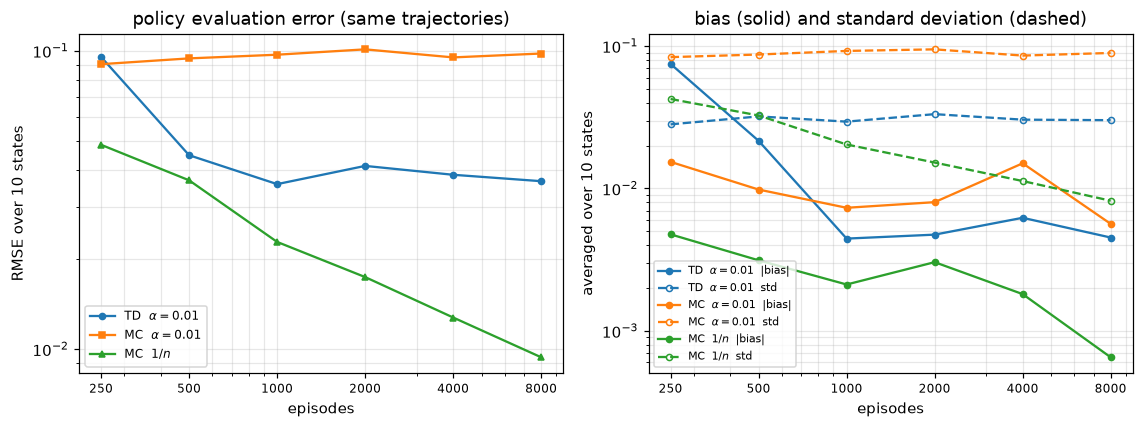
\includegraphics[width=\linewidth]{fig_td_bias_var.png}
\caption{왼쪽: 세 방법의 RMSE. 고정값 $\alpha$를 쓰는 두 방법은 일찍 바닥에 닿아 더 내려가지
않고 $1/n$ 평균만 계속 내려간다. 오른쪽: 같은 실험을 편향(실선)과 표준편차(점선)로 나눈 것.
TD법의 파란 실선이 $250$ 에피소드에서 가장 높은 자리에서 시작해 가파르게 떨어지는 것이
부트스트래핑의 편향이 걷히는 모습이고, 파란 점선이 주황 점선의 $3$분의 $1$ 자리에 가로놓인 것이
분산의 차이다. \texttt{ch06/paper/fig\_td.py}에서 생성.}
\label{fig:bias-var}
\end{figure}

세 번째 열 묶음이 앞 장이 쓴 $1/n$ 평균이다. 고정값 $\alpha$를 쓰는 앞의 둘은 각각 $0.036$과
$0.098$에서 멈추는 반면 $1/n$ 평균만 $8{,}000$ 에피소드까지 계속 내려간다. 예제가 쓰는 설정끼리
견주면 $1{,}000$ 에피소드에서 TD법 $0.0358$ 대 MC법 $0.0229$로 MC법이 앞서는데, 이것이 TD법과
MC법의 우열이 아니라 고정값 $\alpha$와 $1/n$ 평균의 우열이라는 것은 $\alpha$를 맞춘 가운데 열
묶음이 보여 준다.

\subsection{SARSA의 화살표를 만든 것}
\label{app:sarsa-alpha}

본문의 [보충] ``그림 \ref{fig:sarsa-result}의 화살표는 안전한 길이 아니다''가 쓴 근거다. 먼저
SARSA가 수렴해야 할 곳을 표본 없이 계산한다. 앞 장의 정책 반복법을 $\varepsilon$-소프트 정책으로
제한해 돌리면 얻어진다.

\begin{table}[htbp]
\centering
\caption{$\varepsilon$-소프트 정책 가운데 가장 좋은 것이 각 칸에서 고르는 행동. 모두 정책 반복법을
수렴할 때까지 돌려 얻은 정확한 값이며 표본이 섞이지 않았다. 오른쪽 두 열은 문제의 칸 $(2,2)$에서
두 행동의 가치다.}
\label{tab:eps-soft}
\small
\begin{tabular}{@{}lcccrr@{}}
\toprule
$\varepsilon$ & $(2,1)$ & $(2,2)$ & $(1,2)$ & $q((2,2),\texttt{UP})$ & $q((2,2),\texttt{LEFT})$ \\
\midrule
$0$ (순수 탐욕)  & \texttt{RIGHT} & \texttt{UP}   & \texttt{UP} & $0.8100$ & $0.6561$ \\
$0.1$ (예제 값)  & \texttt{RIGHT} & \texttt{UP}   & \texttt{UP} & $0.7684$ & $0.6077$ \\
$0.3$            & \texttt{RIGHT} & \texttt{UP}   & \texttt{UP} & $0.6575$ & $0.4877$ \\
$0.5$            & \texttt{RIGHT} & \texttt{UP}   & \texttt{UP} & $0.4894$ & $0.3282$ \\
$0.7$            & \texttt{LEFT}  & \texttt{UP}   & \texttt{UP} & $0.2288$ & $0.1616$ \\
$0.9$            & \texttt{LEFT}  & \texttt{LEFT} & \texttt{UP} & $-0.1664$ & $-0.0471$ \\
\bottomrule
\end{tabular}
\end{table}

예제가 쓰는 $\varepsilon=0.1$에서 $(2,2)$의 최선은 \texttt{UP}이고 \texttt{LEFT}보다 $0.16$
앞선다. $\varepsilon$을 $0.5$까지 올려도 순서가 바뀌지 않고, 뒤집히려면 $0.9$는 되어야 한다.
곧 원서가 읽은 ``위험 회피''로는 화살표가 설명되지 않는다. 원인을 하나씩 없애 보면 갈린다.

\begin{table}[htbp]
\centering
\caption{$(2,2)$에서 \texttt{UP}을 고른 시드의 수(시드 $20$개). ``자기 목표 기준 RMSE''는 $v_*$가
아니라 표~\ref{tab:eps-soft}에 있는 $\varepsilon$-소프트 최적 가치를 기준으로 한 것이므로, SARSA가
\emph{자기가 수렴해야 할 곳}에 얼마나 이르렀는지를 나타낸다.}
\label{tab:sarsa-cause}
\small
\begin{tabular}{@{}lrrrr@{}}
\toprule
설정 & $(2,2)$에서 \texttt{UP} & $(2,2)$ 방문 & $\max_a Q(2,2)$ & 자기 목표 기준 RMSE \\
\midrule
기본($10{,}000$ 에피소드, $\alpha=0.8$) & $2/20$  & $378$    & $0.3514$ & $0.2389$ \\
에피소드 $20$배($200{,}000$)            & $2/20$  & $5{,}134$ & $0.3353$ & $0.2203$ \\
$\alpha=0.1$                            & $17/20$ & $6{,}089$ & $0.6624$ & $0.1777$ \\
$\alpha=0.1$ + $200{,}000$ 에피소드     & $17/20$ & $42{,}287$& $0.7211$ & $0.0464$ \\
시작 상태를 무작위로($\alpha=0.8$)      & $11/20$ & $3{,}249$ & $0.6640$ & $0.1323$ \\
\bottomrule
\end{tabular}
\end{table}

경험을 $20$배로 늘려도 $2/20$ 그대로다. 표본이 모자란 것이 아니다. $\alpha$를 $0.1$로 낮추면 같은
$10{,}000$ 에피소드에서 $17/20$로 뒤집히고, 거기에 에피소드를 늘리면 $\max_a Q(2,2)$가 목표값
$0.7684$에 다가가며 자기 목표 기준 RMSE가 $0.2389$에서 $0.0464$로 떨어진다. 범인은 $\alpha=0.8$이다.

남은 것은 잔차 띠의 폭이다. $\alpha=0.8$이면 계수 $\sqrt{\alpha/(2-\alpha)}$가 $0.8165$이고,
여기에 TD 목표가 흔들리는 폭 $\sigma_{\text{목표}}$가 곱해진다.

\begin{table}[htbp]
\centering
\caption{수렴한 $Q$에서 TD 목표의 표준편차. SARSA의 목표
$R_t + \gamma Q(S_{t+1},A_{t+1})$에는 $A_{t+1} \sim \varepsilon$-탐욕이라는 뽑기가 들어 있고,
Q 러닝의 목표 $R_t + \gamma\max_a Q(S_{t+1},a)$에는 뽑기가 없다. 환경의 전이가 결정적이라
$R_t$와 $S_{t+1}$은 $(s,a)$가 정해지면 확정이다.}
\label{tab:target-sigma}
\small
\begin{tabular}{@{}lrr@{}}
\toprule
 & SARSA & Q 러닝 \\
\midrule
$(s,a)$ $40$개에 대한 $\sigma_{\text{목표}}$ 평균 & $0.0580$ & $0$ \\
그 최댓값                                          & $0.1708$ & $0$ \\
$\alpha=0.8$에서 예상되는 잔차 띠(평균)            & $0.0473$ & $0$ \\
\bottomrule
\end{tabular}
\end{table}

\begin{figure}[htbp]
\centering
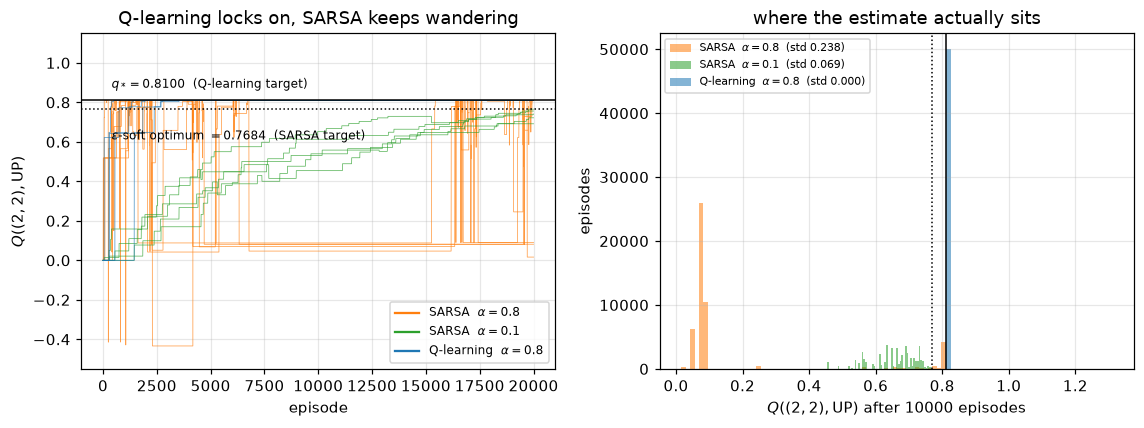
\includegraphics[width=\linewidth]{fig_td_alpha.png}
\caption{왼쪽: $Q((2,2),\texttt{UP})$이 학습 중에 움직이는 모습을 시드 다섯 개씩 겹쳐 그린 것.
파란 선(Q 러닝)은 $q_*=0.8100$에 붙은 뒤 떨어지지 않고, 주황 선(SARSA $\alpha=0.8$)은 위아래로
$1$이 넘는 폭을 오간다. 초록 선($\alpha=0.1$)은 느리지만 점선으로 표시한 자기 목표 $0.7684$를
향해 올라간다. 오른쪽: $10{,}000$ 에피소드 이후 그 값이 실제로 머무는 자리의 분포. Q 러닝은
$0.8100$ 한 점에 못 박혀 막대가 하나뿐이다. \texttt{ch06/paper/fig\_td.py}에서 생성.}
\label{fig:alpha-trace}
\end{figure}

$(2,2)$에서 \texttt{UP}을 골랐을 때의 $\sigma_{\text{목표}}$는 $0.1470$이므로 예상 띠는
$0.8165 \times 0.1470 = 0.1200$이다. $10{,}000$ 에피소드 이후의 값을 모아 실제로 재 보면
표준편차가 $0.2381$로 예상보다 $2$배 가까이 넓다. 앞 장에서도 측정값이 이론값의 $1.5$배 남짓으로
나왔는데, 이론이 표본들의 독립을 가정하는 데 비해 실제로는 목표값 자신이 학습 중에 계속 움직이기
때문이다. $\alpha$를 $0.1$로 낮추면 같은 값이 $0.0691$로 좁아지고, Q 러닝에서는 $0.0000$이다.
두 행동의 차이 $0.16$이 $0.2381$ 안에 묻힌다는 것이 화살표의 정체다.

\subsection{\texorpdfstring{$\rho$}{rho}의 두 형태와 그 분포}
\label{app:rho-place}

본문의 [보충] ``$\rho$를 곱하는 자리''가 쓴 근거다. 예제 형태
$\rho(R_t + \gamma Q')$와 교과서 형태 $R_t + \gamma\rho Q'$를 같은 조건에서 견주었다.

\begin{table}[htbp]
\centering
\caption{두 목표 형태를 시드 $50$개로 견준 것. 갱신식의 나머지는 모두 같다.}
\label{tab:target-form}
\small
\begin{tabular}{@{}lrrrr@{}}
\toprule
목표 & 최적 행동 & $10/10$ & $\max_s|\max_a Q - v_*|$ & RMSE \\
\midrule
$\rho(R_t + \gamma Q')$ (예제)     & $8.36/10$ & $22\%$ & $0.6199$ & $0.2885$ \\
$R_t + \gamma\rho Q'$ (교과서)     & $8.46/10$ & $22\%$ & $0.6270$ & $0.2932$ \\
\bottomrule
\end{tabular}
\end{table}

차이가 시드 사이의 흔들림에 묻힌다. 까닭은 $\rho$가 취하는 값의 분포에 있다.

\begin{table}[htbp]
\centering
\caption{한 걸음 가중치 $\rho$가 실제로 취한 값(시드 $0$, $10{,}000$ 에피소드, 갱신 $136{,}813$회).
대상 정책이 결정적이고 행동 정책이 $\varepsilon$-탐욕이라 값이 사실상 넷뿐인 것은 앞 장 [보충]과
같다. $1.0$은 아직 갱신되지 않아 두 정책이 모두 초기 균등분포인 칸이고, $40$은 두 번의
\lstinline|greedy_probs()| 호출이 동점을 다르게 푼 경우다.}
\label{tab:rho-dist}
\small
\begin{tabular}{@{}lrrl@{}}
\toprule
$\rho$ & 횟수 & 비율 & 언제 \\
\midrule
$1.081$ & $117{,}234$ & $85.69\%$ & $A_{t+1}$이 두 정책의 탐욕 행동일 때 \\
$1.0$   & $10{,}014$  & $7.32\%$  & 두 정책이 아직 균등분포일 때 \\
$0$     & $9{,}564$   & $6.99\%$  & $A_{t+1}$이 $\pi$의 탐욕 행동이 아닐 때 \\
$40$    & $1$         & $0.00\%$  & 동점을 두 호출이 다르게 풀었을 때 \\
\bottomrule
\end{tabular}
\end{table}

$\rho=0$이 되는 것은 갱신의 $6.99\%$뿐이다. 한 걸음짜리 $\rho$가 $0$이 되려면 $A_{t+1}$이 탐욕
행동이 아니어야 하고 $\varepsilon$-탐욕 정책에서 그 확률은 $\varepsilon \cdot 3/4 = 7.5\%$이므로,
실측한 $6.99\%$가 거기에 맞는다. 앞 장 MC법에서 같은 값이 $59.9\%$였던 것은 누적곱이라 한 걸음만
어긋나도 앞선 걸음이 전부 죽었기 때문이다. 두 형태가 실제로 갈리는 것은 $\rho=0$이면서 보상이
$0$이 아닌 갱신뿐인데, 그런 갱신이 $136{,}813$회 가운데 $23$회다.

\subsection{미끄러짐을 넣었을 때}
\label{app:exact}

본문의 [보충] ``오차 $0.00$은 환경이 준 것''이 쓴 근거다. 고른 행동이 정해진 확률로 네 행동 가운데
무작위로 바뀌게 해 두고 같은 실험을 반복하였다.

\begin{table}[htbp]
\centering
\caption{전이에 미끄러짐을 넣었을 때(시드 $50$개, $10{,}000$ 에피소드, $\alpha=0.8$). ``미끄러짐
$10\%$''는 고른 행동이 $10\%$의 확률로 네 행동 가운데 무작위로 바뀐다는 뜻이다. 기준 $v_*$는
미끄러짐이 없는 환경의 값이라 미끄러짐을 넣은 두 줄의 오차에는 환경이 달라진 몫도 섞여 있다.
읽으려는 것은 오차의 크기가 아니라 정확히 $0$인 시드가 사라진다는 것이다.}
\label{tab:slip}
\small
\begin{tabular}{@{}lrrr@{}}
\toprule
환경 & 오차가 정확히 $0$인 시드 & $\max_s|\max_a Q - v_*|$ & 최적 행동 \\
\midrule
결정적(원래 예제) & $43/50$ & $0.0674$ & $9.66/10$ \\
미끄러짐 $10\%$   & $0/50$  & $0.5140$ & $7.42/10$ \\
미끄러짐 $30\%$   & $0/50$  & $0.7320$ & $7.08/10$ \\
\bottomrule
\end{tabular}
\end{table}

미끄러짐을 $10\%$만 넣어도 정확히 맞는 시드가 하나도 남지 않는다. TD 목표에 뽑기가 생겨
$\sigma_{\text{목표}}$가 $0$이 아니게 되고, $\alpha=0.8$의 계수 $0.8165$가 곱해질 상대가 생기기
때문이다.

\subsection{방문하지 않은 칸이 남기는 오차}
\label{app:exact-one}

본문의 [보충] ``하필 $1.0000$인 오차''가 쓴 근거다. 샘플 모델 판본을 에피소드 수만 바꾸어 돌렸다.

\begin{table}[htbp]
\centering
\caption{샘플 모델 판본을 에피소드 수만 바꾸어 돌린 것(시드 $50$개). ``한 번도 방문되지 않은 칸''은
$10{,}000$번의 걸음 동안 그 칸에 한 번도 서 보지 못한 시드의 수다.}
\label{tab:untouched}
\small
\begin{tabular}{@{}lrrr@{}}
\toprule
 & $1{,}000$ 에피소드 & $10{,}000$ 에피소드 \\
\midrule
$\max_s|\max_a Q - v_*|$ 의 평균        & $0.8485$ & $0.1132$ \\
그 값이 정확히 $1.0000$인 시드          & $24/50$  & $0/50$ \\
오차가 가장 큰 칸이 $(1,3)$인 시드      & $25/50$  & $2/50$ \\
오차가 가장 큰 칸이 $(2,3)$인 시드      & $23/50$  & $48/50$ \\
$(1,3)$을 한 번도 방문하지 않은 시드    & $24/50$  & $0/50$ \\
$(2,3)$을 한 번도 방문하지 않은 시드    & $41/50$  & $0/50$ \\
\bottomrule
\end{tabular}
\end{table}

$1.0000$인 시드의 수 $24$와 $(1,3)$을 한 번도 밟지 않은 시드의 수 $24$가 같다. 오차가 참값과 딱
떨어지는 것은 그 칸의 $Q$가 초깃값 $0$에 그대로 남아 있다는 뜻이며, 에피소드를 $10{,}000$으로
늘리면 방문하지 않은 칸과 함께 사라진다.

% =============================================================================
\section*{재현 정보}
\addcontentsline{toc}{section}{재현 정보}
% =============================================================================

본고의 수치는 세 갈래에서 나왔다.

\emph{정확한 값}(표~\ref{tab:eps-soft}, 표~\ref{tab:target-sigma}, 그리고 $v_*$와 $v_\pi$)은
표본을 쓰지 않고 계산한 것이다. 그리드 월드의 가치 함수는 앞 장들의 반복적 정책 평가와 가치
반복법을 갱신 폭이 $10^{-14}$ 아래로 떨어질 때까지 돌려 얻었고, $\varepsilon$-소프트 최적 정책은
정책 반복법을 $\varepsilon$-소프트 정책으로 제한해 돌린 것이다. TD 목표의 표준편차는 그렇게 얻은
$Q$에서 $A_{t+1}$에 대한 분산을 직접 계산했다.

\emph{예제 코드의 실측}(표~\ref{tab:summary}, 표~\ref{tab:sarsa-cause}, 표~\ref{tab:target-form},
표~\ref{tab:rho-dist}, 표~\ref{tab:slip}, 표~\ref{tab:untouched})은 \texttt{ch06/}의 예제를
그대로 돌리고 계측만 덧붙인 것이다. 시드는 \lstinline|np.random.seed()|에 $0$부터 차례로 넣었고,
항목 대부분이 $50$개다. 원인을 갈라 보는 표~\ref{tab:sarsa-cause}에는 에피소드를 $200{,}000$까지
늘리는 설정이 있어 계산 시간 때문에 시드가 $20$개이고, 방문 분포와 칸별 오차도 같은 이유로
$20$개다. $\rho$의 분포는 시드 $0$ 하나를 계측한 것이다.

\emph{그림 스크립트의 실측}(표~\ref{tab:bias-var}, 그림~\ref{fig:bias-var},
그림~\ref{fig:alpha-trace})은 \texttt{ch06/paper/fig\_td.py}로 생성한다. 에피소드를 수십만 번
돌려야 해서 환경의 전이를 미리 표로 펼친 빠른 판본을 쓰지만 갱신식과 정책은 예제와 같다. 두 판본이
어긋나지 않는다는 것은 같은 양을 양쪽에서 재어 확인할 수 있다. $1{,}000$ 에피소드 TD 평가의 RMSE가
예제 코드에서 $0.0376$(시드 $50$개), 빠른 판본에서 $0.0358$(시드 $60$개)로 시드 사이의 흔들림
안에서 맞는다.

표~\ref{tab:slip}의 미끄러짐은 예제를 고친 것이 아니라 환경 쪽에 덧붙인 것이다. 에이전트가 고른
행동을 그대로 \lstinline|env.step()|에 넘기지 않고, 정해진 확률로 네 행동 가운데 하나를 새로 뽑아
넘긴다. 갱신식에 들어가는 \lstinline|action|은 에이전트가 고른 쪽이다.

시드를 바꾸면 값이 달라지는 항목과 그렇지 않은 항목을 섞지 않았다. 표에 ``평균''이라 적힌 것은
시드에 따라 흔들리는 값이다.


\begin{thebibliography}{9}
\bibitem{dlfs4}
사이토 고키, \emph{밑바닥부터 시작하는 딥러닝 4: 파이썬으로 구현하는 강화 학습 알고리즘}, 한빛미디어, 2023.
\bibitem{ch05}
sajacaros, \emph{몬테카를로법: 기댓값을 표본 평균으로 바꾸기}, 2026.
\bibitem{sutton}
R.~S. Sutton and A.~G. Barto, \emph{Reinforcement Learning: An Introduction}, 2nd ed., MIT Press, 2018.
\bibitem{sutton88}
R.~S. Sutton, ``Learning to Predict by the Methods of Temporal Differences,''
\emph{Machine Learning}, vol.~3, pp.~9--44, 1988.
\bibitem{watkins}
C.~J. C.~H. Watkins and P.~Dayan, ``Q-learning,'' \emph{Machine Learning}, vol.~8, pp.~279--292, 1992.
\bibitem{rummery}
G.~A. Rummery and M.~Niranjan, \emph{On-line Q-learning Using Connectionist Systems},
Technical Report CUED/F-INFENG/TR 166, Cambridge University Engineering Department, 1994.
\end{thebibliography}

\vspace{4mm}
\noindent\rule{\linewidth}{0.4pt}\\
\footnotesize
본 문서에 실린 그림 중 ``원서 그림''으로 표기한 것은 참고문헌~\cite{dlfs4}의 도판이며, 학습 정리 목적으로
인용하였다. 그 밖의 그림과 표는 본고에서 직접 생성한 것이다.

\end{document}
